\section{Proposed Methods}


\subsection{Skimming}

\begin{frame}{Document Skimming}

\begin{itemize}
  \item This approach is inspired by the fast reading technique "skimming".
  \item<2-> It involves reading while skipping some parts of the text for efficiency.
  \item<3-> Reader attempts to skip the redundant or irrelevant parts.
\end{itemize}

\only<1>{
	\vskip 3.4cm
}

\only<2->{
	\vskip .5cm
	\begin{figure}
		\centering
		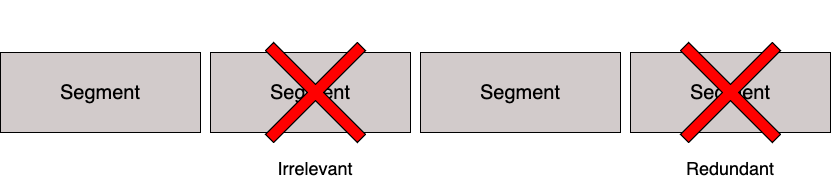
\includegraphics[width=\textwidth]{Images/skim.png}
	\end{figure}
}

\end{frame}

\begin{frame}{Document Skimming (Contd.)}

\begin{itemize}
	\item This method involves uniformly sampling the text segments to fill the LLM's
	context size.
	\item This ensures we capture details from every part of the text.
	\item A similar approach is taken by \citet{wang2024videoagent} for QA on long
	videos.
\end{itemize}

\only<1>{
	\vskip 3cm
}

\only<2->{
	\vskip 1cm
	\begin{figure}
		\centering
		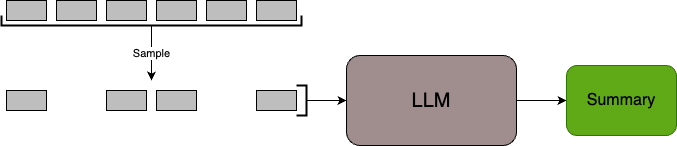
\includegraphics[width=1\textwidth]{Images/doc-skim.png}
	\end{figure}
}

\end{frame}
